\documentclass{article}

% Language setting
% Replace `english' with e.g. `spanish' to change the document language
\usepackage[english]{babel}

% Set page size and margins
% Replace `letterpaper' with `a4paper' for UK/EU standard size
\usepackage[letterpaper,top=2cm,bottom=2cm,left=3cm,right=3cm,marginparwidth=1.75cm]{geometry}

% Useful packages
\usepackage{amsmath}
\usepackage{graphicx}
\usepackage[colorlinks=true, allcolors=blue]{hyperref}

\title{Mathematical proof of the analysis of the cartpole system using Lean4}
\author{Guowei Li}

\begin{document}
\maketitle

\begin{abstract}
This is the final project report for my Advanced Machine Learning course. It demonstrates the use of Lean4 to formally verify the correctness of mathematical derivations. The report first presents a mathematical analysis of the Cartpole system, including modeling the system using Euler-Lagrange mechanics, analyzing the error bounds after local linearization around the equilibrium point, and finally deriving the control law using the LQR (Linear Quadratic Regulator) method and verifying its effectiveness. The second part involves formalizing the above mathematical process in Lean4 and verifying it.
\end{abstract}

\section{Introduction}

\section{System Analysis and Control Method}

\subsection{Cart-Pole Dynamics via Euler--Lagrange Formulation}

We consider a cart of mass $M$ moving horizontally on a frictionless track, with a massless rigid pole of length $l$ and a point mass $m$ attached at its end. The generalized coordinates are chosen as
\[
q_1 = x, \qquad q_2 = \theta,
\]
where $x$ denotes the horizontal position of the cart, and $\theta$ is the pole angle measured from the upright vertical position.

\begin{figure}
\centering
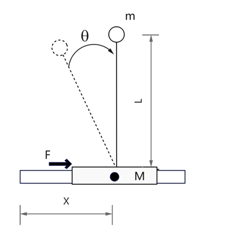
\includegraphics[width=0.4\linewidth]{cartpole.png}
\caption{\label{fig:cartpole}Cartpole System}
\end{figure}

The position of the cart mass is
\[
(x_c,y_c) = (x,0),
\]
and the position of the pole mass (see Fig.~\ref{fig:cartpole}) is
\[
x_p = x - l\sin\theta, \qquad
y_p = l\cos\theta .
\]

The corresponding velocities are
\begin{align}
\dot x_c &= \dot x, \qquad \dot y_c = 0,\\
\dot x_p &= \dot x - l\cos\theta\,\dot\theta,\\
\dot y_p &= -l\sin\theta\,\dot\theta .
\end{align}
Hence the squared speed of the pole mass is
\begin{align}
v_p^2
  &= \dot x_p^2 + \dot y_p^2 \nonumber\\
  &= \bigl(\dot x - l\cos\theta\,\dot\theta\bigr)^2
     + \bigl(-l\sin\theta\,\dot\theta\bigr)^2 \nonumber\\
  &= \dot x^2 - 2 l\dot x\dot\theta\cos\theta + l^2\dot\theta^2.
\end{align}

The kinetic energy of the system is then
\begin{align}
T
  &= \tfrac12 M\dot x^2 + \tfrac12 m v_p^2 \nonumber\\
  &= \frac12 (M+m)\dot x^2
     - m l\dot x\dot\theta\cos\theta
     + \frac12 m l^2\dot\theta^2.
\end{align}

Choosing the potential energy zero at the cart level ($y=0$), the potential energy of the pole mass is
\begin{equation}
V = m g y_p = m g l\cos\theta .
\end{equation}

The Lagrangian is given by
\begin{equation}
L = T - V
  = \frac12 (M+m)\dot x^2
    - m l\dot x\dot\theta\cos\theta
    + \frac12 m l^2\dot\theta^2
    - m g l\cos\theta .
\end{equation}

We now apply the Euler--Lagrange equations
\begin{equation}
\frac{\mathrm{d}}{\mathrm{d}t}\left(\frac{\partial L}{\partial \dot q_i}\right)
 - \frac{\partial L}{\partial q_i}
 = Q_i, \qquad i=1,2,
\end{equation}
where $Q_1 = F$ is the generalized force corresponding to the horizontal input force $F$ on the cart, and $Q_2 = 0$ (no external torque at the pivot).

\paragraph{Equation for $x$.}
The partial derivatives with respect to $\dot x$ and $x$ are
\begin{align}
\frac{\partial L}{\partial \dot x}
&= (M+m)\dot x - m l\dot\theta\cos\theta,\\
\frac{\partial L}{\partial x}
&= 0.
\end{align}
Taking the total time derivative,
\begin{align}
\frac{\mathrm{d}}{\mathrm{d}t}
\left(\frac{\partial L}{\partial \dot x}\right)
&= (M+m)\ddot x
   - m l\bigl(\ddot\theta\cos\theta - \dot\theta^2\sin\theta\bigr) \nonumber\\
&= (M+m)\ddot x
   + m l\sin\theta\,\dot\theta^2
   - m l\cos\theta\,\ddot\theta .
\end{align}
The Euler--Lagrange equation for $x$,
\[
\frac{\mathrm{d}}{\mathrm{d}t}
\left(\frac{\partial L}{\partial \dot x}\right)
- \frac{\partial L}{\partial x} = Q_1 = F,
\]
yields
\begin{equation}
\boxed{ (M+m)\ddot x
       + m l\sin\theta\,\dot\theta^2
       - m l\cos\theta\,\ddot\theta
       = F. }
\label{eq:cart_eq}
\end{equation}

\paragraph{Equation for $\theta$.}
The partial derivatives with respect to $\dot\theta$ and $\theta$ are
\begin{align}
\frac{\partial L}{\partial \dot\theta}
&= - m l\dot x\cos\theta + m l^2\dot\theta,\\
\frac{\partial L}{\partial \theta}
&= m l\dot x\dot\theta\sin\theta + m g l\sin\theta,
\end{align}
where the latter comes from the terms
$- m l\dot x\dot\theta\cos\theta$ and $- m g l\cos\theta$.
Taking the total time derivative of $\partial L/\partial\dot\theta$,
\begin{align}
\frac{\mathrm{d}}{\mathrm{d}t}
\left(\frac{\partial L}{\partial \dot\theta}\right)
&= - m l\ddot x\cos\theta
   + m l\dot x\sin\theta\,\dot\theta
   + m l^2\ddot\theta .
\end{align}
The Euler--Lagrange equation for $\theta$,
\[
\frac{\mathrm{d}}{\mathrm{d}t}
\left(\frac{\partial L}{\partial \dot\theta}\right)
- \frac{\partial L}{\partial \theta} = Q_2 = 0,
\]
gives
\begin{align}
0
&= - m l\ddot x\cos\theta
   + m l\dot x\sin\theta\,\dot\theta
   + m l^2\ddot\theta \nonumber\\
&\quad - \bigl(
   m l\dot x\dot\theta\sin\theta
   + m g l\sin\theta
   \bigr) \nonumber\\
&= - m l\ddot x\cos\theta
   + m l^2\ddot\theta
   - m g l\sin\theta.
\end{align}
Dividing by $m l$ and multiplying by $-1$ yields
\begin{equation}
\boxed{
\ddot x\cos\theta
+ g\sin\theta
- l\ddot\theta
= 0. }
\label{eq:pole_eq}
\end{equation}

Equations~\eqref{eq:cart_eq} and \eqref{eq:pole_eq} together constitute the nonlinear dynamics of the Cart-Pole system under the chosen generalized coordinates and sign conventions.

\subsection{Error Bounds for Cart and Pole Accelerations under Small-Angle Linearization}

We recall the nonlinear Cart--Pole dynamics derived from the Euler--Lagrange formulation.
Define
\[
D(\theta) := M + m\sin^2\theta.
\]
The nonlinear accelerations of the cart and the pole are
\begin{align}
\ddot x_{\mathrm{nl}}
&=
\frac{
F - m l \sin\theta\,\dot\theta^2
 + m g \sin\theta\cos\theta
}{
D(\theta)
},
\label{eq:xddot_nl_def}
\\[2mm]
\ddot\theta_{\mathrm{nl}}
&=
\frac{
F\cos\theta
 - m l \sin\theta\,\dot\theta^2\cos\theta
 + (M+m) g\sin\theta
}{
l\,D(\theta)
}.
\label{eq:thddot_nl_def}
\end{align}

Linearizing around the upright equilibrium
\[
x = 0,\quad \dot x = 0,\quad \theta = 0,\quad \dot\theta = 0,\quad F = 0,
\]
and using
\[
\sin\theta \approx \theta,\qquad
\cos\theta \approx 1,\qquad
\sin^2\theta \approx 0
\]
while neglecting the term proportional to $\sin\theta\,\dot\theta^2$, we obtain the linearized accelerations
\begin{align}
\ddot x_{\mathrm{lin}} &= \frac{F + m g\,\theta}{M},\\[1mm]
\ddot\theta_{\mathrm{lin}} &= \frac{F + (M+m) g\,\theta}{M l}.
\end{align}

We now quantify the approximation error between the nonlinear and linearized accelerations in a small neighbourhood of the upright equilibrium.

\subsubsection*{Assumptions and Small-Angle Bounds}

We restrict attention to a local operating region
\[
|\theta| \le \theta_{\max},\qquad
|\dot\theta| \le \Omega_{\max},\qquad
|F| \le F_{\max},
\]
where we will eventually choose $\theta_{\max} = 5^\circ = 5\pi/180$ (in radians).
From $\sin^2\theta \ge 0$ it follows that
\begin{equation}
M \,\le\, D(\theta) \,\le\, M + m,
\qquad
\frac{1}{M+m} \,\le\, \frac{1}{D(\theta)} \,\le\, \frac{1}{M}.
\label{eq:D_bounds}
\end{equation}

Standard Taylor expansions of the trigonometric functions yield, for all $|\theta|\le\theta_{\max}$,
\begin{align}
|\sin\theta - \theta|
&\le \frac{\theta_{\max}^3}{6}, \label{eq:sin_err}\\
|\cos\theta - 1|
&\le \frac{\theta_{\max}^2}{2}, \label{eq:cos_err}\\
|\sin^2\theta|
&\le \theta_{\max}^2, \label{eq:sin2_err}
\end{align}
and $|\sin\theta| \le |\theta| \le \theta_{\max}$.

\subsubsection*{Error Bound for Cart Acceleration}

Define the cart acceleration error
\[
\Delta_x := \ddot x_{\mathrm{nl}} - \ddot x_{\mathrm{lin}}.
\]
Substituting \eqref{eq:xddot_nl_def} and the linearized expression, we obtain
\begin{align}
\Delta_x
&= F\Bigl(\frac{1}{D(\theta)} - \frac{1}{M}\Bigr)
 + m g\Bigl(\frac{\sin\theta\cos\theta}{D(\theta)}
            - \frac{\theta}{M}\Bigr)
 - \frac{m l\sin\theta\,\dot\theta^2}{D(\theta)}.
\end{align}

We bound each term separately.

\paragraph*{(i) Denominator linearization error (force term).}
Using~\eqref{eq:D_bounds} and~\eqref{eq:sin2_err},
\[
\Bigl|\frac{1}{D(\theta)} - \frac{1}{M}\Bigr|
= \frac{|M - D(\theta)|}{M D(\theta)}
= \frac{m\sin^2\theta}{M D(\theta)}
\le \frac{m\theta_{\max}^2}{M^2},
\]
hence
\begin{equation}
\Bigl|
F\Bigl(\frac{1}{D(\theta)} - \frac{1}{M}\Bigr)
\Bigr|
\le
\frac{m}{M^2}\,F_{\max}\,\theta_{\max}^2.
\label{eq:x_err_force}
\end{equation}

\paragraph*{(ii) Trigonometric linearization error (gravity term).}
We write
\[
\frac{\sin\theta\cos\theta}{D(\theta)} - \frac{\theta}{M}
=
\underbrace{\frac{\sin\theta\cos\theta - \theta}{D(\theta)}}_{(a)}
+
\underbrace{\theta\Bigl(\frac{1}{D(\theta)} - \frac{1}{M}\Bigr)}_{(b)}.
\]

For term (a), using~\eqref{eq:sin_err}, \eqref{eq:cos_err} and $|\sin\theta|\le\theta_{\max}$,
\begin{align}
|\sin\theta\cos\theta - \theta|
&\le |\sin\theta - \theta|
    + |\sin\theta||\cos\theta - 1| \nonumber\\
&\le \frac{\theta_{\max}^3}{6}
    + \theta_{\max}\frac{\theta_{\max}^2}{2}
 = \Bigl(\frac{1}{6} + \frac{1}{2}\Bigr)\theta_{\max}^3
 = \frac{2}{3}\theta_{\max}^3.
\end{align}
Using $D(\theta)\ge M$,
\[
|(a)| \le \frac{2}{3}\frac{\theta_{\max}^3}{M}.
\]

For term (b), using the bound on $1/D(\theta) - 1/M$,
\[
|(b)|
\le \theta_{\max}\frac{m\theta_{\max}^2}{M^2}
= \frac{m}{M^2}\theta_{\max}^3.
\]

Combining,
\[
\Bigl|
\frac{\sin\theta\cos\theta}{D(\theta)} - \frac{\theta}{M}
\Bigr|
\le
\theta_{\max}^3\left(
\frac{2}{3M} + \frac{m}{M^2}
\right),
\]
and thus
\begin{equation}
\Bigl|
m g\Bigl(\frac{\sin\theta\cos\theta}{D(\theta)} - \frac{\theta}{M}\Bigr)
\Bigr|
\le
m g\,\theta_{\max}^3
\left(
\frac{2}{3M} + \frac{m}{M^2}
\right).
\label{eq:x_err_trig}
\end{equation}

\paragraph*{(iii) Neglected nonlinear centrifugal term.}
Using $D(\theta)\ge M$ and $|\sin\theta|\le\theta_{\max}$,
\begin{equation}
\Bigl|\frac{m l\sin\theta\,\dot\theta^2}{D(\theta)}\Bigr|
\le \frac{m l\theta_{\max}}{M}\,\dot\theta^2
\le \frac{m l}{M}\,\theta_{\max}\,\Omega_{\max}^2.
\label{eq:x_err_omega}
\end{equation}

\paragraph*{Summary for $\ddot x$.}
Collecting \eqref{eq:x_err_force}, \eqref{eq:x_err_trig} and \eqref{eq:x_err_omega}, we obtain
\begin{equation}
\boxed{
|\ddot x_{\mathrm{nl}} - \ddot x_{\mathrm{lin}}|
\;\le\;
\frac{m}{M^2}F_{\max}\,\theta_{\max}^2
\;+\;
m g\,\theta_{\max}^3\Bigl(
\frac{2}{3M} + \frac{m}{M^2}
\Bigr)
\;+\;
\frac{m l}{M}\,\theta_{\max}\,\Omega_{\max}^2.
}
\label{eq:x_error_bound}
\end{equation}

\subsubsection*{Error Bound for Pole Angular Acceleration}

Define the angular acceleration error
\[
\Delta_\theta := \ddot\theta_{\mathrm{nl}} - \ddot\theta_{\mathrm{lin}}.
\]
From \eqref{eq:thddot_nl_def} and the linearized expression,
\begin{align}
\Delta_\theta
&=
\frac{F\cos\theta}{l D(\theta)}
 - \frac{F}{M l}
 - \frac{m l\sin\theta\,\dot\theta^2\cos\theta}{l D(\theta)}
 + \frac{(M+m) g\sin\theta}{l D(\theta)}
 - \frac{(M+m) g\,\theta}{M l} \nonumber\\
&=: A + B + C,
\end{align}
where we group the terms as
\begin{align}
A &:= \frac{F\cos\theta}{l D(\theta)} - \frac{F}{M l},\\
B &:= - \frac{m l\sin\theta\,\dot\theta^2\cos\theta}{l D(\theta)}
    = -\frac{m\sin\theta\,\dot\theta^2\cos\theta}{D(\theta)},\\
C &:= \frac{(M+m) g\sin\theta}{l D(\theta)}
      - \frac{(M+m) g\,\theta}{M l}.
\end{align}

\paragraph*{(i) F term (A).}
We have
\[
\frac{\cos\theta}{D(\theta)} - \frac{1}{M}
=
\frac{\cos\theta - 1}{D(\theta)}
+ \Bigl(\frac{1}{D(\theta)} - \frac{1}{M}\Bigr),
\]
so using~\eqref{eq:cos_err} and the bound on $1/D(\theta) - 1/M$,
\[
\Bigl|\frac{\cos\theta}{D(\theta)} - \frac{1}{M}\Bigr|
\le
\frac{\theta_{\max}^2}{2M} +
\frac{m\theta_{\max}^2}{M^2}.
\]
Therefore
\begin{equation}
|A|
= \frac{|F|}{l}\Bigl|\frac{\cos\theta}{D(\theta)} - \frac{1}{M}\Bigr|
\le
\frac{F_{\max}}{l}\left(
\frac{\theta_{\max}^2}{2M} +
\frac{m\theta_{\max}^2}{M^2}
\right).
\label{eq:theta_err_force}
\end{equation}

\paragraph*{(ii) Neglected nonlinear term (B).}
Using $D(\theta)\ge M$, $|\sin\theta|\le\theta_{\max}$ and $|\cos\theta|\le 1$,
\begin{equation}
|B|
\le \frac{m\theta_{\max}}{M}\,\dot\theta^2
\le \frac{m}{M}\,\theta_{\max}\,\Omega_{\max}^2.
\label{eq:theta_err_omega}
\end{equation}

\paragraph*{(iii) Gravity term (C).}
We write
\[
C = \frac{(M+m) g}{l}
\Bigl(\frac{\sin\theta}{D(\theta)} - \frac{\theta}{M}\Bigr),
\]
and decompose
\[
\frac{\sin\theta}{D(\theta)} - \frac{\theta}{M}
=
\underbrace{\frac{\sin\theta - \theta}{D(\theta)}}_{(a)}
+
\underbrace{\theta\Bigl(\frac{1}{D(\theta)} - \frac{1}{M}\Bigr)}_{(b)}.
\]
From~\eqref{eq:sin_err} and $D(\theta)\ge M$,
\[
|(a)| \le \frac{\theta_{\max}^3}{6M},
\]
and from the bound on $1/D(\theta) - 1/M$,
\[
|(b)| \le \theta_{\max}\frac{m\theta_{\max}^2}{M^2}
= \frac{m}{M^2}\theta_{\max}^3.
\]
Thus
\[
\Bigl|\frac{\sin\theta}{D(\theta)} - \frac{\theta}{M}\Bigr|
\le \theta_{\max}^3\left(
\frac{1}{6M} + \frac{m}{M^2}
\right),
\]
and hence
\begin{equation}
|C|
\le
\frac{(M+m) g}{l}\,
\theta_{\max}^3\left(
\frac{1}{6M} + \frac{m}{M^2}
\right).
\label{eq:theta_err_trig}
\end{equation}

\paragraph*{Summary for $\ddot\theta$.}
Collecting \eqref{eq:theta_err_force}, \eqref{eq:theta_err_omega} and \eqref{eq:theta_err_trig}, we obtain
\begin{equation}
\boxed{
|\ddot\theta_{\mathrm{nl}} - \ddot\theta_{\mathrm{lin}}|
\;\le\;
\frac{F_{\max}}{l}\left(
\frac{\theta_{\max}^2}{2M} +
\frac{m\theta_{\max}^2}{M^2}
\right)
\;+\;
\frac{m}{M}\,\theta_{\max}\,\Omega_{\max}^2
\;+\;
\frac{(M+m) g}{l}\,
\theta_{\max}^3\left(
\frac{1}{6M} + \frac{m}{M^2}
\right).
}
\label{eq:theta_error_bound}
\end{equation}

\subsubsection*{Interpretation}

Equations~\eqref{eq:x_error_bound} and~\eqref{eq:theta_error_bound} show that, for bounded input $F$ and angular velocity $\dot\theta$ and for sufficiently small angle range $|\theta|\le\theta_{\max}$, the errors between the nonlinear accelerations and their linearized counterparts are uniformly bounded by quantities of order
\[
\mathcal{O}(\theta_{\max}^2) + \mathcal{O}(\theta_{\max}^3)
 + \mathcal{O}(\theta_{\max}\Omega_{\max}^2).
\]
In particular, for $\theta_{\max} = 5^\circ$ the trigonometric linearization errors are extremely small, and the dominant contribution arises from the neglected nonlinear centrifugal term proportional to $\theta_{\max}\Omega_{\max}^2$. This justifies the use of the linearized Cart--Pole model for LQR design within the specified small-angle operating region.

\subsection{Design of Control Law Using LQR}


\section{Verification of the Mathematical Process Using Lean4}


\bibliographystyle{alpha}


\end{document}
